\chapter{Anforderungen an das Projekt}

 Es soll eine Verwaltungs-Software für RFID-Karten entwickelt werden, die in einem Schließfach aufbewahrt werden. Die Admin-Anwendung organisiert die Karten im Schließfach, über die Client-Anwendung  können berechtigte Nutzer Karten reservieren, ausleihen und zurückgeben. Eine REST-API dient als Schnittstelle zwischen der Hardware und den Anwendungen.
\subsection{Anforderungen}
\begin{itemize}
    \item Quaderförmiges Gehäuse mit wenig Bauhöhe zu der Wand. (ME)
    \item Zentrales Display. (IT)
    \item Entnahmeregistrierung mit Buchungszeile am Display. (IT)
    \item Schließfächer für mind. 10 Karten. (ME)
    \item Kartenverwaltung (je Automat). (IT)
    \item Jedes Schließfach soll transparent sein. (ME)
    \item Jede Karte soll stehend parallel zur Wand sichtbar sein. (ME)
    \item Jedes Schließfach soll elektrisch aufspringen. (ME)
    \item Jedes Schließfach soll durch Finger druck wieder geschlossen werden. (ME)
    \item Rückgabe-Kontrolle der Karte nur am richtigen Fach. (IT)
    \item Löschung der zugeordneten Buchungszeile am Display. (IT)
    \item Datenverwaltung für Statistik im Hintergrund. (IT)
    \item Administrativer Wartungszugang. (IT)
\end{itemize}

\section{Komponenten}

\subsection{Grafische Darstellung des Gesamtsystems}
\begin{center}
\includegraphics[width=0.95\textwidth]{MJ/assets/complete-system.png}
\captionof{figure}{Zusammenspiel der Komponenten des Systems}
\end{center}

\subsubsection{REST-API}
Die REST-API ist der zentrale Knotenpunkt zum Austausch von Daten zwischen Client-, Display- und Admin Anwendung (Flutter App) und den Schließfächern. Die REST-API kommuniziert mit den Schließfächern mithilfe des MQTT Protokolls, welche jeweils ein Topic zugewiesen bekommen und so Daten senden, als auch empfangen können. Die REST-API speichert etwaige Daten in der MySQL Datenbank. Diese Daten können ausschließlich von der REST-API verwaltet werden. Gehostet wird die REST-API und Datenbank auf einem zentralen Server, sodass der Zugriff auf die ebenfalls zentralisierte Datenbank vereinfacht wird und alle Daten konsistent sind.

\subsubsection{Login – Anwendung}
Die Anmeldung der Lehrkräfte erfolgt über die O365 Authentifizierung. Es ist nur über diese Funktion möglich, auf die Anwendung zuzugreifen. Um den Anmeldeprozess zu beschleunigen, gibt es die "Remember me"-Funktion, die es Lehrkräften ermöglicht, sich automatisch bei zukünftigen Besuchen der Anwendung anzumelden, ohne jedes Mal ihre Anmeldedaten eingeben zu müssen.

Bei der Neuregistrierung einer Lehrkraft wird ihre Karte gescannt.
  
\subsubsection{Client – Anwendung}
Die Client-Anwendung ist eine benutzerfreundliche Smartphone-App, die speziell für Lehrer entwickelt wurde. Nach einer erfolgreichen Anmeldung können Lehrer mithilfe der App Karten reservieren und ausleihen. Die App bietet eine schnelle und einfache Möglichkeit, den Bestand an verfügbaren Karten zu durchsuchen und zu überprüfen, welche Karten bereits ausgeliehen sind.
  
\subsubsection{Display – Anwendung}
Die Anwendung wird auf dem Display des Tresors angezeigt und dient als visuelle Unterstützung bei verschiedenen Aktionen. Mit dieser Anwendung können alle Reservierungen eingesehen werden und es ist auch möglich, eine Karte direkt anzufordern.


\subsubsection{Admin – Anwendung}
Die Admin-Anwendung soll dazu verwendet werden können, administrative Aufgaben erledigen zu können. Diese Anwendung soll auch als Webseite und APP zur Verfügung stehen, um solche Einstellungen nicht direkt Vorort machen zu müssen. Die Admin-App wird mit Flutter erstellt. Um die Admin-App benutzen können, muss ein Benutzer ein Admin sein.


\subsection{Schnittstellen}
\subsubsection{Kommunikation zwischen App und REST-API}
Die Client bzw. Admin Anwendung auf dem Endgerät des Benutzers als auch auf dem Display des Schließfaches kommunizieren mittels der oben beschriebenen REST-API miteinander. 

\subsubsection{Kommunikation zwischen REST-API und Cardstorage Unit}
Die Schließfächer kommunizieren mit der REST-API mithilfe des MQTT Protokolls. Das Controller-Programm, welches auf dem Raspberry (bzw. ein anderer Mikroprozessor) eines Schließfaches läuft, kommuniziert mit der REST-API, um die Kommandos, welche die REST-API von dem Client bzw. Admin Anwendung erhält, auszuführen.

\subsection{Zielbestimmung}
    \textbf{Muss-Ziele}: Diese Ziele müssen unbedingt erreicht werden, um das Projekt erfolgreich abzuschließen oder um bestimmte rechtliche oder regulatorische Anforderungen zu erfüllen. Muss-Ziele werden immer mit dem Wort \textbf{`muss'} formuliert.\\

    \textbf{Wunsch- oder Kann-Ziele}: Diese Ziele sind optional und je nach verfügbarer Zeit und Ressourcen erreicht werden können. Wunsch- oder Kann-Ziele werden mit \textbf{`soll'} oder \textbf{`kann'} formuliert.

\subsubsection{Zentrale REST-API}
Die Zentrale REST-API erfüllt folgende Kriterien:
\begin{itemize}
    \item Die Nutzer der API m\"ussen über die REST-API Benutzer, Karten, und Schlie\ss f\"acher anlegen, abrufen, ändern und löschen können
    \item Die Nutzer der API m\"ussen die Möglichkeit haben über die REST-API Karten als reserviert und wieder zurückgegeben zu melden
    
    \item Die REST-API muss zwischen Administrator und Benutzer unterscheiden

    \item Die Nutzer der API sollen Daten zur statistischen Auswertung durch den Administrator abrufen können (Häufigkeiten von Reservierungen von Karten etc.)

    \item Die Nutzer der API sollen Daten für Informationszwecken abrufen können (API-Logs: Zugriffe von Clients, etc.)

    \item Die REST-API soll als Softwarepaket in Form eines portablen Docker-Containers zur Verfügung stehen

\end{itemize}

\subsubsection{API -- Raspberry Kommunikation}
Die Kommunikation zwischen zentraler REST-API und Raspberry erfüllt folgende Kriterien 
\begin{itemize}
    \item Die Nutzer der API tauschen etwaige Daten mit der REST-API über MQTT aus
    \item Die Nutzer der API tauschen etwaige Daten mit dem Python Programm aus, welche die Motoren des Schließfaches und dem Kartenleser steuert.
\end{itemize}

\subsubsection{Login – Anwendung}
\begin{itemize}
  \item Der Benutzer muss sich mittels seinem Microsoft Account einloggen
  \item Der Benutzer muss bei der Registrierung, ein Schlie\ss fach ausw\"ahlen und dort seine Karte scannen lassen.
  \item Der Benutzer soll die Möglichkeit haben seinen Login zu speichern.
    \item Der Benutzer soll beim Login die Möglichkeit haben, Fragen an den Admin zu stellen

\end{itemize}

\subsubsection{Client - Anwendung}
\begin{itemize}

    \item Die Client-Anwendung muss ein direktes Anfordern einer Karte erm\"oglichen

    \item Die Client-Anwendung muss ein Reservierungssystem f\"ur die Karten bieten

    \subitem Reservierungen m\"ussen bearbeitbar/l\"oschbar sein

    \subitem Reservierungen sollen eine Benachrichtigung bei einem bevorstehenden Termin versenden


    \item Die Client-Anwendung soll die Möglichkeit bieten bestimmte Karte zu favorisieren 

    
    \item Die Client-Anwendung soll eine Benachrichtigung versenden, falls eine markierte Karte wieder frei geworden ist.

    \item Die Client-Anwendung soll eine Einstellungsseite bieten (Benachrichtigungen, Thememode, Account, Abmelden)
    \item Die Client-Anwendung soll ein System zum Chatten mit anderen Lehrern bieten, falls diese eine ben\"otigte Karte in Verwendung haben

    \item Die Client-Anwendung soll die Möglichkeit bieten, Nachrichten an den Admin zu senden (Feedback, Verbesserungen […])
\end{itemize}

\subsubsection{Admin – Anwendung}
Die Anforderungen an die Admin-App gestalten sich folgendermaßen:
\begin{itemize}
  \item Der Admin muss Karten anlegen / löschen / bearbeiten können.
  \item Der Admin muss Karten und Schließfächer anlegen / löschen / bearbeiten können.
  \item Der Admin muss Benutzer löschen können.
  \item Der Admin muss Benutzer zu Admin machen können.
  \item Der Admin muss Reservierungen löschen können.
  \item Der Admin muss die späteste Abholzeit der Reservierung einstellen können.
  \item Der Admin soll Statistiken anzeigen lassen können.
  \item Der Admin soll Logs anzeigen lassen können.
\end{itemize}

\subsubsection{Display – Anwendung}
\begin{itemize}
    \item Die Display-Anwendung muss auf einem Raspberry PI angezeigt werden, der mit dem Bildschirm eines Schließfachs verbunden ist.
    \item Die Display-Anwendung muss das Beantragen einer Karte erm\"oglichen.
    \item Die Display-Anwendung sollte in der Lage sein, alle Reservierungen der Karten im entsprechenden Schließfach anzuzeigen.
    \item Die Display-Anwendung sollte die verbleibende Zeit bis zum Scannen einer Karte anzeigen, zum Beispiel für Registrierung oder Authentifizierung.
\end{itemize}

\newpage

\subsection{Use-Case Diagramme}

\begin{figure}[h!]
  \centering
  \includegraphics[width=1\textwidth]{FLUTTER/images/GP/login-use-case.png}
  \caption{Use-Case Login-Sicht \cite{Flutter-Architektur-SVG}}
\end{figure}
\newpage

\begin{figure}[h!]
  \centering
  \includegraphics[width=1\textwidth]{FLUTTER/images/GP/client-use-case.png}
  \caption{Use-Case Client-Sicht \cite{Flutter-Architektur-SVG}}
\end{figure}
\newpage

\begin{figure}[h!]
  \centering
  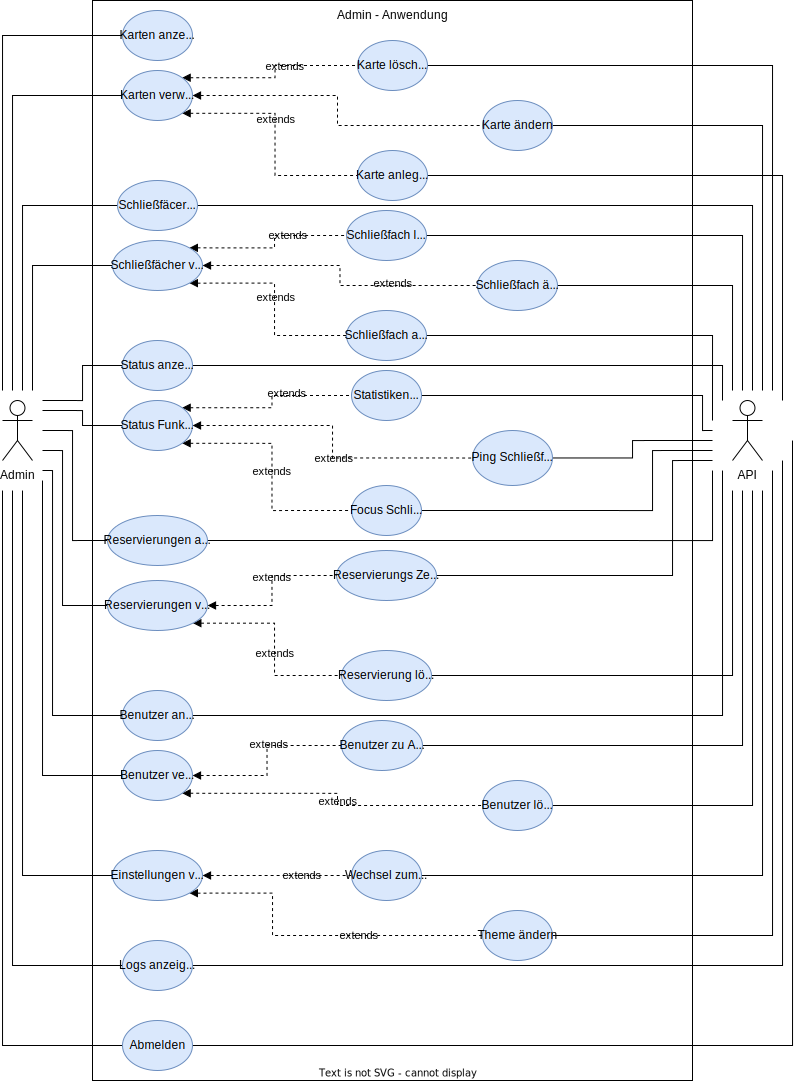
\includegraphics[width=0.92\textwidth]{FLUTTER/images/ZB/admin_use_case.png}
  \caption{Use-Case Admin-Sicht \cite{Flutter-Architektur-SVG}}
\end{figure} 
\newpage

\begin{figure}[h!]
  \centering
  \includegraphics[width=1\textwidth]{FLUTTER/images/GP/display-use-case.png}
  \caption{Use-Case Display-Sicht \cite{Flutter-Architektur-SVG}}
\end{figure} 

%\begin{figure}[h!]
 % \centering
 % \vspace{0.5cm}
 % \includegraphics[width=1\textwidth]{FLUTTER/images/GP/Use-Case.png}
 %   \caption{Use Case Diagramm der zu erstellenden Software}
%\end{figure}

\newpage

\section{Meilensteine}
\begin{itemize}
    \item 01.11.2022 Admin-Anwendung v1 abgeschlossen
    \item 01.11.2022 Client-Anwendung v1 abgeschlossen
    \item 01.11.2022 Display-Anwendung v1 abgeschlossen
    \item 01.11.2022 REST-API/DB v1 abgeschlossen
    
    \item 02.02.2023 Admin-Anwendung v2 abgeschlossen
    \item 02.02.2023 REST-API/DB v2 abgeschlossen
    \item 02.02.2023 Client-Anwendung v2 abgeschlossen
    \item 02.02.2023 Display-Anwendung v2 abgeschlossen

    \item 28.02.2023 Raspberry-API Kommunikation abgeschlossen
    \item 28.02.2023 Dokumentation abgeschlossen
    \item 30.04.2023 Abschluss Test durchgeführt 
\end{itemize}